\documentclass[10pt,letterpaper]{article}
\usepackage[utf8]{inputenc}
\usepackage{amssymb, amsmath}
\usepackage{graphicx}
\usepackage{fancyhdr}
\usepackage{multicol}
\usepackage{multirow}
\usepackage{float}
\usepackage{wrapfig}
\usepackage{graphicx}

\usepackage{hyperref}
\renewcommand{\refname}{}
\hypersetup{
    colorlinks=true,
    linkcolor=red,
    filecolor=magenta,      
    urlcolor=blue,
    citecolor=blue,
}


\graphicspath{ {img1/} }


\usepackage[letterpaper,top=2cm,bottom=2cm,left=3cm,right=3cm,marginparwidth=1.75cm]{geometry}





\fancyhf{}
\lhead[\leftmark]{}
\rhead[]{César Ornelas}
\lfoot[\thepage]{}
\rfoot[]{\thepage}



\begin{document}

\begin{title}

\begin{wrapfigure}{r} %this figure will be at the right
    \centering
    
\includegraphics[width=4cm]{img/logos.png}
\end{wrapfigure}

Octubre 2024
\begin{center}
    \vspace{1cm}
    \hspace{1cm}
    \Large
    \textbf{Densímetros} \\

    \vspace{0.5cm}

    \normalsize
    López Gónzalez A. , Hernández Gómez A. \\ Villanueva Sanluis A. , Ornelas Arias C.
    
    \vspace{0.3cm}

\end{center}
    

    
    
\end{title}

    \hline
	\section*{Resumen}

    En este trabajo se presentan los resultados obtenidos mediante dos métodos experimentales para la determinación de la densidad de diversos fluidos. El primer método emplea un densímetro casero, mientras que el segundo utiliza un dinamómetro para medir la fuerza de flotación ejercida sobre un objeto sumergido en los fluidos. El objetivo es comparar los valores de densidad obtenidos por ambos procedimientos y evaluar su congruencia. Se diseñó y calibró el densímetro utilizando aceite y agua como líquidos de referencia, estableciendo una relación lineal entre la densidad del fluido y la profundidad de inmersión. Por otro lado, el método del dinamómetro se basó en el principio de Arquímedes, registrando las fuerzas actuantes al sumergir un balín en diferentes fluidos. A pesar de que los resultados de ambos métodos no coinciden exactamente, las incertidumbres asociadas permiten afirmar que existe consistencia entre ellos. Finalmente, se discuten las limitaciones de los equipos utilizados y se proponen mejoras en la precisión para futuros experimentos, como la construcción de densímetros más finos y el uso de dinamómetros más sensibles.


    \vspace{1cm}

    \hline
	
    \section{Introducción}

    \hline
    
    \begin{multicols}{2}

    \subsection*{Marco Teórico}

La determinación de la densidad de un fluido se basa en principios fundamentales de la física clásica, específicamente en el principio de Arquímedes y en el concepto de flotabilidad. Estos principios permiten desarrollar diversos métodos experimentales para medir la densidad, tanto utilizando instrumentos específicos, como un densímetro, como a partir de la fuerza de flotación experimentada por un objeto sumergido en el fluido.

\subsubsection*{Principio de Arquímedes}

El principio de Arquímedes establece que todo cuerpo sumergido total o parcialmente en un fluido experimenta una fuerza hacia arriba, conocida como fuerza de empuje o flotación, que es igual al peso del fluido desplazado por el cuerpo. Matemáticamente, esta fuerza de empuje \( F_b \) se expresa como:

\begin{equation}
F_b = V \rho_f g
\end{equation}

donde \( V \) es el volumen del objeto sumergido, \( \rho_f \) es la densidad del fluido, y \( g \) es la aceleración gravitacional. Este principio es fundamental para la determinación de densidades en el presente experimento, ya que permite relacionar el peso de un objeto en el aire con la fuerza que experimenta al estar sumergido en un fluido.

\subsubsection*{Densímetro: Método basado en la flotabilidad}

Un densímetro es un instrumento que mide la densidad de un fluido basado en el principio de flotación. El funcionamiento del densímetro está gobernado por la ecuación de flotación, donde la profundidad a la que se hunde el densímetro dentro del fluido depende de la densidad del fluido en cuestión. El concepto subyacente es que el peso del densímetro es equilibrado por la fuerza de empuje del fluido desplazado, de manera que para cada fluido el nivel de inmersión del densímetro varía.

En este caso particular, el densímetro fue construido de manera improvisada utilizando el tubo de una pluma y plastilina para darle estabilidad. La ecuación teórica que relaciona la profundidad de inmersión \( y \) con la densidad \( \rho \) del fluido es lineal:

\begin{equation}
\rho = my + b
\end{equation}

donde \( m \) es la pendiente obtenida mediante la calibración con fluidos de densidad conocida, y \( b \) es la ordenada al origen, que en este caso se corresponde con la densidad del agua, utilizada como referencia. Esta relación lineal permite determinar la densidad de otros fluidos, como el aceite, el jabón y la glicerina, al medir la profundidad de inmersión del densímetro en dichos líquidos.

\subsubsection*{Método del dinamómetro: Fuerza de flotación}

El segundo método experimental para medir la densidad de un fluido consiste en sumergir un objeto, en este caso un balín, en el fluido y medir la fuerza que ejerce el fluido sobre el objeto utilizando un dinamómetro. Al suspender el balín en el aire, el dinamómetro registra su peso \( W \), mientras que al sumergirlo en un fluido, el dinamómetro mide una fuerza \( F_i \) que es menor que \( W \) debido a la fuerza de empuje que actúa sobre el balín. La relación entre estas fuerzas y la densidad del fluido se describe mediante la ecuación de Arquímedes:

\begin{equation}
W = F_b + F_i = V \rho_f g + F_i
\end{equation}

Despejando la densidad del fluido \( \rho_f \), obtenemos la siguiente relación:

\begin{equation}
\rho_f = \frac{W - F_i}{V g}
\end{equation}

Donde \( V \) es el volumen del balín (suponiendo que es conocido o medido previamente). Esta ecuación describe cómo la diferencia entre el peso del balín en el aire y la fuerza medida por el dinamómetro cuando está sumergido en el fluido permite calcular la densidad del fluido.

\subsubsection*{Comparación entre ambos métodos}

Ambos métodos se basan en principios teóricos sólidos y bien establecidos. El densímetro se apoya directamente en la relación entre el volumen de fluido desplazado y la densidad, mientras que el método del dinamómetro utiliza el principio de Arquímedes para relacionar la fuerza de flotación con la densidad del fluido. En ambos casos, se espera que los valores obtenidos para la densidad sean consistentes, dentro de los márgenes de error experimentales, debido a que ambos dependen de la fuerza de empuje del fluido.

La ventaja del método del densímetro radica en la simplicidad de su construcción y operación, siempre que el dispositivo esté bien calibrado. El método del dinamómetro, por otro lado, tiene la ventaja de ser más directo al medir la fuerza de flotación y depender menos de la geometría del objeto utilizado, aunque está más sujeto a las incertidumbres del dinamómetro.


    \begin{figure}[H]
        \centering
        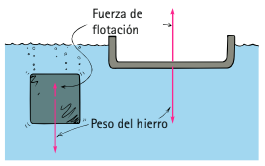
\includegraphics[width = 5cm]{img/img2.png}
        \caption{\label{flot} Un bloque de hierro se hunde, mientras que la misma
        cantidad de hierro con forma de tazón flota. \cite{hamb}}
    \end{figure}    

    

    

    \subsection{Objetivos}

    Se pretende obtener de dos formas experimentales distintas, una  la densidad de varios fluidos. Para el primero se construirá un densímetro, y para el segundo, colgando un objeto de un dinamómetro, se va a sumergir los distintos fluidos para compararlo con la medida obtenida de su peso al colgarlo simplemente.

    \subsection{Hipótesis}

    Se espera que haya congruencia con ambos métodos, de tal forma que las densidades obtenidas sean similares.


    
    \end{multicols}




    \vspace{1cm}

    \hline

    \section{Desarrollo}

    \hline

    \begin{multicols}{2}

    \subsection{Construcción del densímetro}

    \subsubsection{Materiales}

    \begin{itemize}
        \item Bolígrafo / Pluma
        \item Plastilina
        \item Vernier
        \item Masking tape
        \item Aceite
        \item Glicerina
        \item Jabón
    \end{itemize}
    

   \subsubsection{Armado y funcionamiento del densímetro}

    Se tenia previsto utilizar un densímetro con un popote y plastilina, ya calibrado, que por un infortunio ya no se pudo utilizar, lo que nos obligo a armar en ese momento otro. Un diagrama de este se muestra en la figura \ref{F1}. Este fue construido con el tubo de una pluma, vació, con un trozo de plastilina debajo para
    darle estabilidad al sumergirlo.

    \begin{figure}[H]
        \centering
        
\includegraphics[width = 4cm]{img/img1.png}
        \caption{}
        \label{F1}
    \end{figure} 

    Dado que para aquel momento, resultaba complicado establecer una escala, el principio de funcionamiento es el siguiente: Tenemos que, siempre que sea el tubo y no la parte con plastilina la que este sobre la interfaz del fluido y el aire, la relación entre la densidad y cuanta distancia se sumerge es lineal. De esta forma, fijando un eje de coordenadas paralelo al tubo, pegando masking en el tubo, el valor $y$ en el que se ubica la interfaz, se relacionará de la siguiente forma con la densidad:

    \begin{equation}
        \label{eq:relin}
        \rho = my + b
    \end{equation}

    Podemos  obtener los parámetros de la eq \ref{eq:relin} si conocemos la posición $y$ de dos fluidos, y sus densidades.
    (para la eq de una recta solo se requiere conocer dos pares $(y, \rho)$). Donde, siendo esos líquidos aceite y agua, y $\rho_o, \rho_a$ sus densidades.

    \begin{equation}
        \label{eq:m}
        m = \frac{\rho_a - \rho_o}{y_a - y_o}
    \end{equation}

    Para obtener el valor de $b$ hace falta primero establecer donde se va a colocar el origen del eje de coordenadas. Si por comodidad elegimos que sea en el punto donde se obtiene la interfaz al sumergirlo en agua ($y_a = 0$), por la eq \ref{eq:relin} tendremos que:

    \begin{equation}
        \label{eq:b}
        b = \rho_a
    \end{equation}

    Consideramos para todas las posiciones de las interfaces de cada fluido, que si esta se encuentra debajo de la del agua, tendrá valores positivos, mientras que si se encuentra arriba, tendrá valores negativos. En la figura \ref{F2} se muestran las posiciones
    de interfaz de los 4 fluidos, y al lado un Vernier para establecer una escala en milímetros de $y$

    \begin{figure}[H]
        \centering
        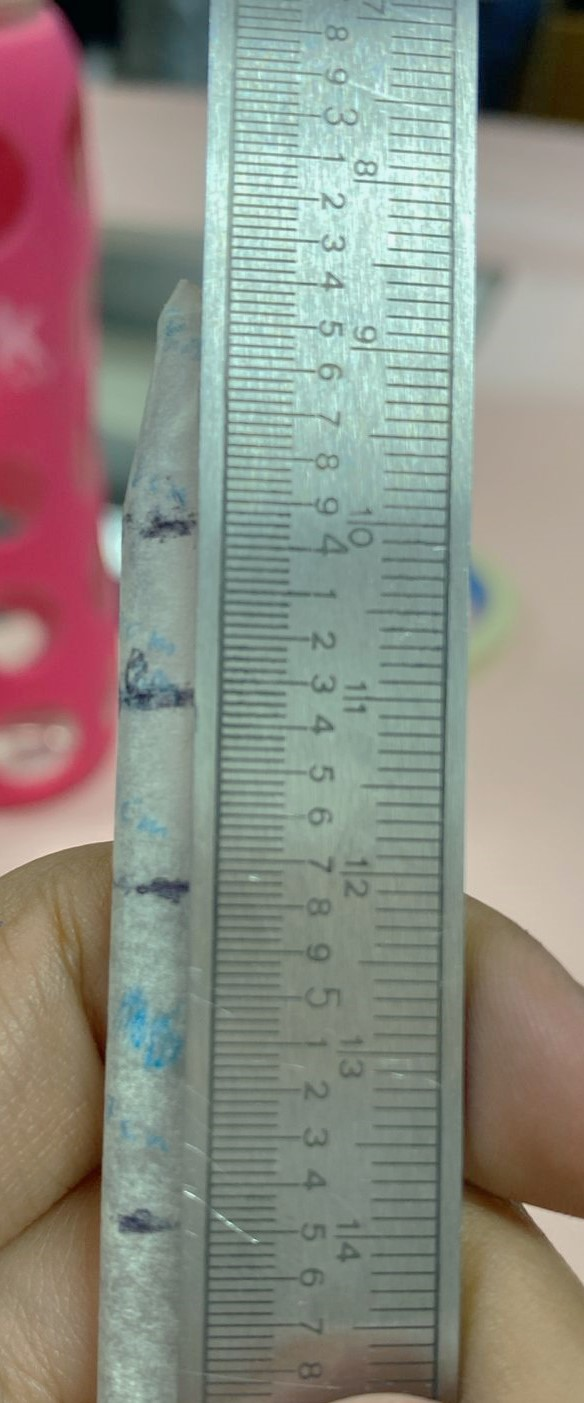
\includegraphics[width = 4cm]{img/dens.jpg}
        \caption{}
        \label{F2}
    \end{figure} 

    
    \subsection{Densidad con dinamómetros}

     \subsubsection{Materiales}

    \begin{itemize}
        \item Cordón
        \item Balín
        \item Dinamómetro
        \item Aceite
        \item Glicerina
        \item Jabón
    \end{itemize}
    

   \subsubsection{Toma de densidades}

    Se suspendió el balín simplemente sobre el aire para obtener el peso que se registraba. Posteriormente se sumergió en agua, aceite, glicerina, y Jabón, y se registraron los valores de fuerza dados por el dinamómetro.  
    Del principio de Arquimedes tenemos que la fuerza boyante es: $F_b = V \rho_i g$ donde $V$ es volumen del balín, $\rho_i$ la densidad del medio, y $g$ la fuerza de gravedad. Sea $W$ el peso registrado al colgar el balín solo, y $F_i$ la fuerza registrada por el dinamómetro al momento se sumergir, tenemos que: $W = F_b + F_i = V \rho_i g + F_i$.
    
    Si despejamos $\rho_i$ para escribirla en términos de $F_i$, llegamos a que: $\rho_i = - F_i (1/gV) + W/gV$. Lo que nos debe importar ahora, es que si observamos bien, tenemos una eq lineal que podemos escribir como:

    \begin{equation}
        \label{eq:m2}
        \rho = F_i m + b
    \end{equation}

    Donde solo hace falta conocer dos pares de datos para encontrar $m$, y que para una densidad de $0$ \footnote{Aunque prácticamente todo esta sumergido en el aire, al ser muy pequeña su densidad, se ignora}, el dinamómetro marca el valor $W$. De la misma forma, con la medida del dinamómetro al sumergirlo en agua, y conociendo la densidad del agua, podemos obtener los parámetros de la eq \ref{eq:m2}

    

    

    \subsection{Análisis de los datos}

    \subsubsection{Densímetro}

    En el software de tracker se analizo la imagen de la fig \ref{F2} para obtener los valores $y$ de las interfaces. Se considera una incertidumbre de apreciación de medio milímetro para cada una, y los datos se muestran en la tabla \ref{tab1}

    \begin{table}[H] 
    \caption{\label{tab1} Posiciones de interfaces} 
       \begin{center}
       \begin{tabular}{|p{2cm}|p{3cm}|}
       \hline
        Aceite & $- (9.8 \pm 0.5)$mm \\
       \hline
        Agua & $0$ mm\\
       \hline
        Jabón & $(11 \pm 0.5)$mm \\
        \hline
        Glicerina & $(30.2 \pm 0.5)$mm \\
        \hline
       \end{tabular}
       \end{center}
    \end{table}

    Ahora bien, el valor que tenemos registrado para la densidad del
    agua es de $(999 \pm 2)$kg/m$^3$, mientras que el del aceite, que
    era de coco y girasol, tomando en cuenta el rango de cada uno \cite{aceite}, tenemos que es de $916 \pm 8$kg/m$^3$. Considerando lo anterior, la eq \ref{eq:m}, y su propagación de incertidumbres, llegamos a que: $m = (8.5 \pm 1.2)$ kg/(m$^3$ mm) (Si bien $m$ tiene en el denominador de sus unidades metros y milímetros, al multiplicar por los valores de la tabla \ref{tab1}, los milímetros se eliminan), por lo que nuestra eq queda como: (considerando las unidades como kg/(m$^3$)
    
    \begin{equation}
        \label{eq:lindens}
        \rho = (8.5 \pm 1.2) y +  (999 \pm 2)
    \end{equation}

    Por lo que con los datos de la tabla \ref{tab1} encontramos que las densidades del jabón y la glicerina son $(1092.5 \pm 19.5)$ kg/m$^3$ y
    $(1255.7 \pm 42.5)$ kg/m$^3$, respectivamente.






    \subsubsection{Dinamómetro}

    Las fuerzas registradas por el dinamómetro fueron en los distintos medios fueron:

    \begin{table}[H] 
    \caption{\label{tab2} Pesos registrados} 
       \begin{center}
       \begin{tabular}{|p{2cm}|p{3cm}|}
       \hline
        Aire & $ (0.1375 \pm 0.0025)$N \\
       \hline
        Aceite & $(0.06 \pm 0.0025)$N \\
       \hline
        Agua & $(0.0525 \pm 0.0025)$ N\\
       \hline
        Jabón & $(0.0475 \pm 0.0025)$N \\
        \hline
        Glicerina & $(0.0325 \pm 0.0025)$N \\
        \hline
       \end{tabular}
       \end{center}
    \end{table}    

    Utilizando la eq \ref{eq:m2}, tomando la densidad del aire como $O$, y la del agua como $(999 \pm 2)$kg/m$^3$, junto con los datos de la tabla anterior, tenemos que $m = (-11752 \pm 27)$ kg/(m$^3$ N). Consideremos escribir la eq de la recta de la forma punto pendiente, sabiendo que para la fuerza registrada en el aire $W$ (el peso), consideramos que la densidad es 0. Entonces:

    \begin{equation}
        \label{lindin}
        \rho = (-11752 \pm 27) (F_d - W)
    \end{equation}

    Donde $F_d$ son las fuerzas tabuladas en la tabla \ref{tab2}. Con lo anterior los datos que encontramos para las densidades son:

    \begin{table}[H] 
    \caption{\label{tab2} Densidades} 
       \begin{center}
       \begin{tabular}{|p{1.8cm}|p{3.2cm}|}
       \hline
        Aceite & $(910 \pm 31)$ kg/m$^3$  \\
       \hline
        Jabón & $(1057 \pm 32)$ kg/m$^3$ \\
        \hline
        Glicerina & $(1233.96 \pm 32)$ kg/m$^3$ \\
        \hline
       \end{tabular}
       \end{center}
    \end{table} 



    

    \end{multicols}


    \vspace{0.7cm}    

    \hline

    \section{Resolución}

    \hline

    \begin{multicols}{2}
    
        \subsection{Conclusión: }

        AL comparar los datos obtenidos por ambos métodos, si bien numéricamente no pudiesen estar tan cerca como esperábamos, las incertidumbres (sobre todo las del segundo método) son suficientes para que estos valores lleguen a cubrirse, y podamos afirmar que hay congruencia en ambos métodos. Notese también que el valor para la densidad del aceite en el segundo método se aproxima bastante al teórico que se utilizó para el primero. Si bien los valores obtenidos resultan ser congruentes, se siguiere utilizar herramientas mas precisas en futuras ocasiones para obtener datos mas precisos. Esto podría obtenerse si se usara un densímetro mas fino, y un dinamómetro mas sensible. 

        \subsection{Bibliografía}
    
        \begin{thebibliography}{9}
        \bibitem{hamb} Hewitt, P. G. (2016). Física Conceptual. 12 Ed. Pearson.
        \bibitem{aceite} T. (2023) Cuál es la densidad del aceite: aceite vegetales y minerales?. EspacioCiencia. Recuperado de \url{https://espaciociencia.com/cual-es-la-densidad-del-aceite/} 

        \end{thebibliography}


    \end{multicols}
            
    \hline

    \vspace{1cm}

  
	
\end{document}